
\documentclass[11pt,a4paper]{article}

\usepackage[T1]{fontenc}
\usepackage[utf8]{inputenc}
\usepackage{lmodern}
\usepackage[margin=2.2cm]{geometry}
\usepackage{amsmath,amssymb,mathtools}
\usepackage{enumitem}
\usepackage{tikz}
\usetikzlibrary{arrows.meta,positioning}

\setlength{\parindent}{0pt}
\setlength{\parskip}{0.5em}

\newcommand{\N}{\mathbb{N}}
\newcommand{\eps}{\varepsilon}
\newcommand{\trans}[1]{\xrightarrow{#1}}
\newcommand{\bis}{\mathrel{\sim}}
\newcommand{\appn}[1]{\mathrel{\sim_{#1}}}

\begin{document}

\begin{center}
{\large Z. 2026 \qquad CONCURRENCY THEORY \qquad P. Hofman}

\vspace{0.4em}
{\Large \textbf{Tutorial 4}}

\vspace{0.2em}
\textbf{Bisimilarity on infinite-state systems}
\end{center}

\medskip

\textbf{Conventions.}
All transition systems in this sheet use strong transitions.
For a labelled transition system, $\sim$ denotes strong bisimilarity.
A relation $R$ is a bisimulation if every move from either side can be
matched by a move with the same label, leading again to a pair in $R$.

For vectors we use componentwise addition and the componentwise order on
$\N^k$.  A set is \emph{semilinear} if it is a finite union of linear sets.

% ---------------------------------------------------------------------------

\section*{A. A finite warm-up}

\textbf{Exercise 1. [Compute bisimilarity]}
Consider the following finite LTS.

\begin{center}
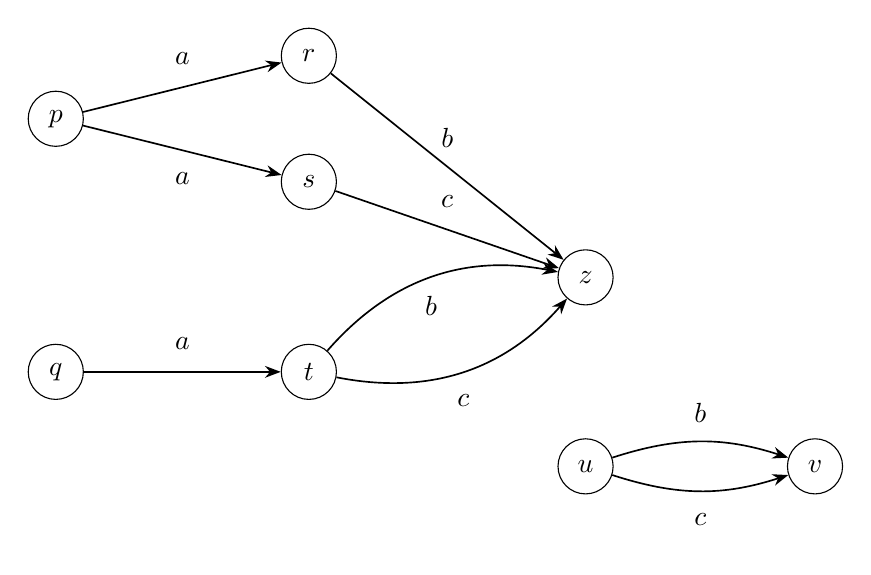
\begin{tikzpicture}[
  >=Stealth,
  node distance=15mm and 22mm,
  every node/.style={circle,draw,minimum size=7mm,inner sep=1pt},
  every edge/.style={draw=black,line width=0.6pt,-{Stealth[length=2mm]}}
]
\node (p) {$p$};
\node (q) [below=25mm of p] {$q$};

\node (r) [right=25mm of p, yshift=8mm] {$r$};
\node (s) [right=25mm of p, yshift=-8mm] {$s$};
\node (t) [right=25mm of q] {$t$};

\node (z) [right=28mm of t, yshift=12mm] {$z$};
\node (u) [right=28mm of t, yshift=-12mm] {$u$};
\node (v) [right=22mm of u] {$v$};

\draw (p) edge node[draw=none,above] {$a$} (r);
\draw (p) edge node[draw=none,below] {$a$} (s);
\draw (q) edge node[draw=none,above] {$a$} (t);

\draw (r) edge node[draw=none,above] {$b$} (z);
\draw (s) edge node[draw=none,above] {$c$} (z);

\draw (t) edge [bend left] node[draw=none,below] {$b$} (z);
\draw (t) edge [bend right] node[draw=none,below] {$c$} (z);

\draw (u) edge[bend left=18] node[draw=none,above] {$b$} (v);
\draw (u) edge[bend right=18] node[draw=none,below] {$c$} (v);
\end{tikzpicture}
\end{center}

\begin{enumerate}[label=(\alph*)]
\item Compute all bisimulation equivalence classes.
\item Decide whether $p\sim q$.
\item Give a winning first move for Spoiler from $(p,q)$.
\item Give an HML formula which is true in exactly one of $p,q$.
\item Compute the first few approximants $\sim_0,\sim_1,\ldots$ until the
      pair $(p,q)$ disappears.
\end{enumerate}

% ---------------------------------------------------------------------------

\section*{B. Congruences on $\N^k$}

\textbf{Exercise 2. [Congruences are semilinear]}
An equivalence relation $\equiv$ on $\N^k$ is a \emph{congruence} if
\[
    x\equiv y
    \quad\Longrightarrow\quad
    x+z\equiv y+z
    \qquad\text{for every }z\in\N^k.
\]
We identify $\equiv$ with the set
\[
    R_{\equiv}=\{(x,y)\in\N^k\times\N^k:x\equiv y\}
    \subseteq \N^{2k}.
\]

A set $S\subseteq\N^d$ is called a \emph{slice} if
\[
    u,\ u+v,\ u+w\in S
    \quad\Longrightarrow\quad
    u+v+w\in S.
\]

You may use the following theorem of Eilenberg--Sch\"utzenberger:

\medskip
\emph{Every slice $S\subseteq\N^d$ is semilinear.}
\medskip

\begin{enumerate}[label=(\alph*)]
\item Let $\equiv$ be a congruence on $\N^k$.
      Suppose
      \[
      (x,y),\quad (x+p,y+q),\quad (x+r,y+s)
      \]
      belong to $R_{\equiv}$.
      Prove that
      \[
      (x+p+r,y+q+s)\in R_{\equiv}.
      \]

\item Conclude that every congruence on $\N^k$ is a semilinear relation.

\end{enumerate}

\textbf{Optional challenge. [Why are slices semilinear?]}
Let $S\subseteq\N^d$ be a slice.  For $u\in S$ define
\[
  S-u=\{v\in\N^d:u+v\in S\},
  \qquad
  M_u=\bigl(\min((S-u)\setminus\{0\})\bigr)^*,
\]
where $\min X$ denotes the set of componentwise-minimal elements of $X$,
and $A^*$ is the submonoid generated by $A$.

\begin{enumerate}[label=(\alph*)]
\item Use Dickson's lemma to show that every $M_u$ is finitely generated.
\item Show that $u+M_u\subseteq S$.
\item Show that if $u\leq v$ and $M_u=M_v$, then
      \[
          v+M_v\subseteq u+M_u.
      \]
\item Complete the argument that only finitely many sets $u+M_u$ are needed
      to cover $S$.
\end{enumerate}

% ---------------------------------------------------------------------------

\section*{C. BPP: bisimilarity as a congruence}

A BPP has variables $X_1,\ldots,X_k$ and finitely many rules
\[
     X_i \trans{a} \alpha,
     \qquad \alpha\in\N^k.
\]
A configuration is a vector $x\in\N^k$.  A rule above induces
\[
    x \trans{a} x-e_i+\alpha
\]
whenever $x_i>0$ and $e_i$ is a unit vector with $1$ on the component $i$.

\textbf{Exercise 3. [Adding the same process]}
Prove that
\[
      x\sim y
      \quad\Longrightarrow\quad
      x+z\sim y+z
\]
for all BPP configurations $x,y,z$.

\begin{enumerate}[label=(\alph*)]
\item Prove that
\[
x\sim y
\quad\Longrightarrow\quad
x+z\sim y+z
\]
for all BPP configurations $x,y,z$.
\item Using Exercise 2, conclude that BPP bisimilarity is semilinear.
\end{enumerate}

\textbf{Exercise 4. [A symbolic infinite bisimulation]}
Consider the BPP with variables $X,Y,A$ and rules
\[
\begin{array}{rclcrcl}
X &\trans{a}& X+A, &&
Y &\trans{a}& Y+A,\\
X &\trans{b}& 0,   &&
Y &\trans{b}& 0,\\
A &\trans{c}& 0.
\end{array}
\]
Here $+$ denotes multiset union and $0$ is the empty configuration.

\begin{enumerate}[label=(\alph*)]
\item Prove that
      \[
          X+nA \sim Y+nA
          \qquad\text{for every }n\in\N.
      \]
Give one finite description of an infinite bisimulation witnessing all
      these pairs at once.
\end{enumerate}

% ---------------------------------------------------------------------------

\section*{D. Two semi-decision procedures}

For an arbitrary LTS define relations $\sim_n$ by
\[
  \sim_0=S\times S,
\]
and, for $n\geq 0$, let $p\sim_{n+1}q$ if every transition from either
state can be matched by a transition with the same label whose endpoints
are related by $\sim_n$.

\textbf{Exercise 5. [Searching for a negative witness]}
Assume that the LTS is finitely branching.

\begin{enumerate}[label=(\alph*)]
\item Show that, for fixed $p,q,n$, the property $p\sim_n q$ can be decided
      by exploring a finite game tree of depth $n$.
\item Prove
      \[
           p\sim q \quad\Longrightarrow\quad
           p\sim_n q\qquad\text{for every }n.
      \]
\item Prove the converse:
      \[
           \bigl(\forall n\;\; p\sim_n q\bigr)
           \quad\Longrightarrow\quad
           p\sim q.
      \]
      Use K\"onig's lemma on the tree of finite Duplicator strategies.
\item Deduce a semi-decision procedure for $p\not\sim q$.
\end{enumerate}

\textbf{Exercise 6. [Searching for a positive witness in BPP]}
Let $x,y$ be configurations of a fixed BPP.

A semilinear relation $R\subseteq\N^k\times\N^k$ can be represented by a
Presburger formula.  You may use that Presburger arithmetic is decidable
and that semilinear relations can be effectively enumerated.

\begin{enumerate}[label=(\alph*)]
\item Write the one-step condition saying that a relation $R$ is a
      bisimulation.
\item Design a semi-decision procedure for $x\sim y$, use the fact that semi-linear sets are enumerable.

\end{enumerate}

\textbf{Comment. [Decidability from two searches]}
Run the procedures from Exercises 5 and 6 in parallel.
Note that one has to accept thus strong bisimilarity for BPP is decidable.

% ---------------------------------------------------------------------------

\section*{E. Why finite branching matters}

\textbf{Exercise 8. [All finite approximants, but not bisimilar]}
For $m\in\N$, let $C_m$ be a finite $b$-chain of length $m$:
\[
  c_m \trans{b} c_{m-1}\trans{b}\cdots
  \trans{b}c_0,
\]
where $c_0$ has no outgoing transition.
Let $C_\infty$ be the infinite $b$-chain.

Construct states $p,q$ as follows:
\[
  p\trans{a} C_m \quad\text{for every }m\in\N,
\]
and
\[
  q\trans{a} C_m \quad\text{for every }m\in\N,
  \qquad
  q\trans{a} C_\infty.
\]

\begin{enumerate}[label=(\alph*)]
\item Prove that $p\sim_n q$ for every $n\in\N$.
\item Prove that $p\not\sim q$.
\item Identify precisely where the proof of Exercise 5(c) fails.
\end{enumerate}

% ---------------------------------------------------------------------------

\section*{F. Normed BPA}

A BPA has variables $X_1,\ldots,X_k$ and rules
\[
      X\trans{a}\alpha,
      \qquad \alpha\in\{X_1,\ldots,X_k\}^*.
\]
Configurations are words.  The operational rule is
\[
      X\beta\trans{a}\alpha\beta.
\]
The BPA is \emph{normed} if every variable can reach the empty word
$\eps$.

For a configuration $\alpha$, define its norm by
\[
   \|\alpha\|
   =
   \min\{|w|:\alpha\trans{w}\eps\}.
\]

\textbf{Exercise 9. [Norm as a bisimulation invariant]}
Assume that the BPA is normed.

\begin{enumerate}[label=(\alph*)]
\item Prove that every non-empty configuration has an outgoing transition.
\item Prove
      \[
          \|\alpha\beta\|
          =
          \|\alpha\|+\|\beta\|.
      \]
\item Prove that
      \[
          \alpha\sim\beta
          \quad\Longrightarrow\quad
          \|\alpha\|=\|\beta\|.
      \]
\item Construct two normed BPA configurations with the same norm which are
      not bisimilar.
\end{enumerate}

\textbf{Discussion.}
Norm is only the first invariant used by polynomial algorithms for normed
BPA bisimilarity.  A full algorithm needs stronger decomposition properties.
Which additional information, beyond the norm, would be useful when comparing
two long BPA words?

% ---------------------------------------------------------------------------

\section*{G. Summary question}

\textbf{Exercise 10. [What made the decidability proof work?]}
For the BPP argument above, identify the role of each property:

\begin{enumerate}[label=(\roman*)]
\item finite branching;
\item bisimilarity being a congruence;
\item every congruence on $\N^k$ being semilinear;
\item decidability of Presburger arithmetic;
\item dovetailing two semi-decision procedures.
\end{enumerate}

For each item, say which part of the proof would fail without it.


\textbf{Exercise 9. [Norm as a bisimulation invariant]}
Assume that the BPA is normed.

\begin{enumerate}[label=(\alph*)]
	\item Prove that every non-empty configuration has an outgoing transition.
	\item Prove
	\[
	\|\alpha\beta\|
	=
	\|\alpha\|+\|\beta\|.
	\]
	\item Prove that
	\[
	\alpha\sim\beta
	\quad\Longrightarrow\quad
	\|\alpha\|=\|\beta\|.
	\]
	\item Construct two normed BPA configurations with the same norm which are
	not bisimilar.
\end{enumerate}

\textbf{Exercise 10. [Cancellation and prime decomposition]}
A BPA word is called \emph{prime} (up to bisimilarity) if it is non-empty
and is not bisimilar to a product of two non-empty words.
Here products are concatenations, and $\eps$ is the identity.

\begin{enumerate}[label=(\alph*)]
	\item Prove that bisimilarity is a congruence for concatenation:
	$\alpha\sim\beta$ implies $\alpha\gamma\sim\beta\gamma$ and
	$\gamma\alpha\sim\gamma\beta$. Pay attention to termination.
	\item Prove \emph{right cancellation} for normed BPA:
	\[
	\alpha\gamma\sim\beta\gamma\quad\Longrightarrow\quad\alpha\sim\beta.
	\]
	Hint: use a relation of pairs with the same suffix and the fact that a
	non-empty normed prefix can make a move.
	\item Prove \emph{left cancellation}:
	\[
	\gamma\alpha\sim\gamma\beta\quad\Longrightarrow\quad\alpha\sim\beta.
	\]
	Hint: follow a shortest word reducing $\gamma$ to $\eps$.
	\item Explain why normedness is important in these arguments.
\end{enumerate}

\textbf{Exercise 11. [Unique decomposition]}
You may use the following \emph{unique decomposition theorem} for normed
BPA: every configuration is bisimilar to a concatenation of primes, and
the sequence of prime equivalence classes is unique.

\begin{enumerate}[label=(\alph*)]
	\item Prove existence of a prime decomposition by induction on the norm.
	\item Use the theorem to show that, if prime decompositions are known,
	checking bisimilarity of two BPA words reduces to comparing two sequences.
	\item Let $X_1,\ldots,X_k$ be the variables. Explain why it is enough to
	compute prime decompositions of these $k$ variables, rather than of all
	words. How do you decompose a word $X_{i_1}\cdots X_{i_m}$?
	\item Show that every prime appearing in the decomposition of a variable
	has norm at most the norm of that variable. Can the total decomposition
	length exceed the norm?
\end{enumerate}

\textbf{Exercise 12. [A finite decomposition base]}
A \emph{decomposition base} chooses some variables as representatives of
prime classes and gives each remaining variable $X$ a word $d(X)$ over
prime representatives. Extend $d$ to words by concatenation, and let
$\equiv_d$ mean equality of the resulting words:
\[
\alpha\equiv_d\beta\quad\Longleftrightarrow\quad d(\alpha)=d(\beta).
\]

\begin{enumerate}[label=(\alph*)]
	\item Show that $\equiv_d$ is a congruence. Why can one test equality
	modulo $\equiv_d$ without constructing an infinite-state graph?
	\item Write a finite set of conditions on the BPA rules sufficient to
	ensure that $\equiv_d$ is a bisimulation. Explain how to test these
	conditions by comparing normal forms of rule successors.
	\item Suppose $\equiv_d$ is a bisimulation and the base contains the
	input pair $(\alpha,\beta)$ in the sense that
	$d(\alpha)=d(\beta)$. What can you conclude?
	\item Why is checking that a proposed base is a bisimulation easier than
	finding the correct base?
\end{enumerate}

\textbf{Exercise 13. [Towards a polynomial-time algorithm --- challenge]}
Assume that all variables are normed and their norms are available.
The unique decomposition theorem is available as a black box.

\begin{enumerate}[label=(\alph*)]
	\item Order variables by nondecreasing norm. Why can a composite
	variable of norm $n$ only decompose into primes of smaller norm?
	\item Propose how to represent candidate decompositions by a compact
	finite base. Identify the operations needed to compare two words under
	such a base.
	\item A proposed base can be checked by finitely many transition tests.
	Explain why this does \emph{not} by itself prove that a polynomial-time
	algorithm exists.
	\item Research challenge: describe how a decomposition-base refinement
	algorithm avoids enumerating all candidate bases. State what must be
	bounded to obtain polynomial running time.
\end{enumerate}

\textbf{Remark.} The preceding exercises explain why prime decomposition
turns equivalence into a finite algebraic problem. The complete
polynomial-time algorithm for normed BPA requires an additional
polynomial-time base-refinement argument; unique decomposition alone is
not an algorithm for finding the base.

% ---------------------------------------------------------------------------

\section*{G. Summary question}

\textbf{Exercise 14. [What made the decidability proof work?]}
For the BPP argument above, identify the role of each property:

\begin{enumerate}[label=(\roman*)]
	\item finite branching;
	\item bisimilarity being a congruence;
	\item every congruence on $\N^k$ being semilinear;
	\item decidability of Presburger arithmetic;
	\item dovetailing two semi-decision procedures.
\end{enumerate}

For each item, say which part of the proof would fail without it.

\end{document}



